% !TEX root = morphkasten.tex

\section{Kamera}


%##############
\subsection{Raspberry Pi Cam}

\begin{figure}[h!]%Position festigen
\centering
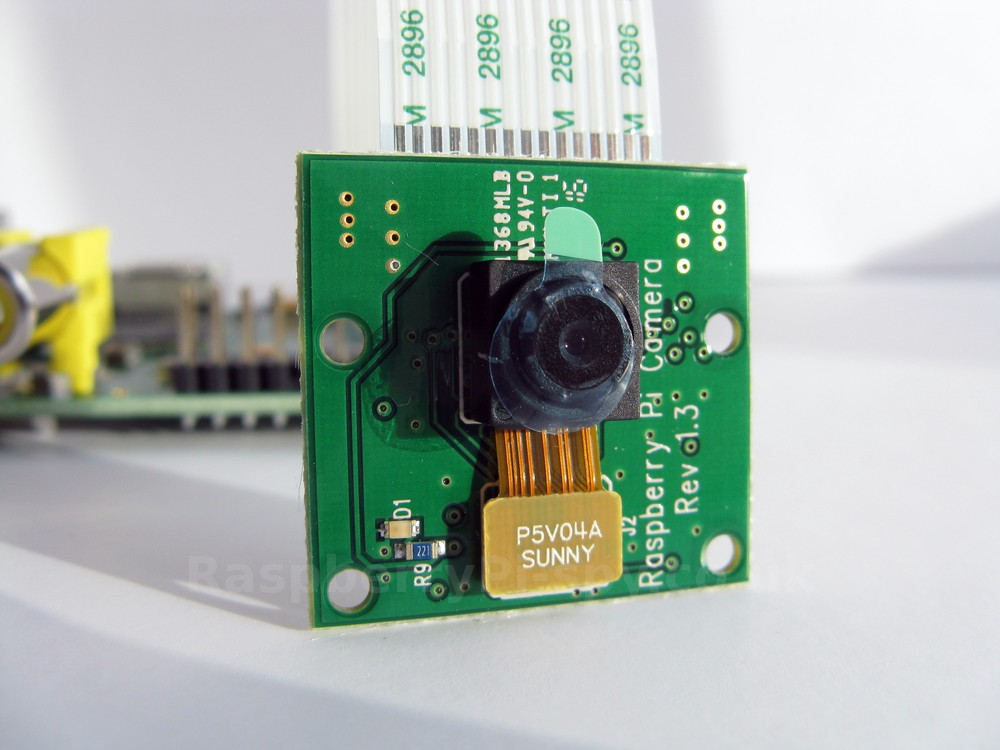
\includegraphics[width=0.5\textwidth]{fig/raspberry-pi-camera-module.jpg}
\caption{Pi Cam (Quelle: https://www.raspberrypi.org)}
\label{fig:PiCam}
\end{figure}

\begin{table}[h]
\begin{tabular}{p{0.5\textwidth} | p{0.5\textwidth}}


 \textbf{Vorteile} & \textbf{Nachteile} \\ \hline
	 
\begin{itemize}
\item Tiefe Anschaffungskosten
\item Kleine Baugrösse
\item Grosse Community
\item OpenSource Treiber
\item Gute Auflösung
\end{itemize}

 
 &
 
\begin{itemize}
\item Fester Fokus auf 1m
\item Relativ geringer Winkel mit 53.5°
\item Halterung muss erstellt werden
\item MIPI Schnittstelle erforderlich
\end{itemize}

\end{tabular}
\end{table}

\begin{table}[h]
\begin{tabular}{p{0.5\textwidth}p{0.5\textwidth}}


 \textbf{Risiken} & \\ \hline
	 
\begin{itemize}
\item Fahrbahn kann in der Kurve nicht vollständig erfasst werden
\item Objekte können nicht vollständig erfasst werden
\item Kompatibilität zu Minicomputer eingeschränkt (Nur Rasp Pi und Banana Pi)
\end{itemize}
&
\begin{itemize}
\item Kein Autofokus: Scharfstellung nicht sichergestellt
\item Farbverhalten bei unterschiedlichen Lichtverhältnissen 
\end{itemize}

 
\end{tabular}
\end{table}

\pagebreak

%##############
\subsection{Raspberry Pi Cam Noir}

\begin{figure}[h!]%Position festigen
\centering
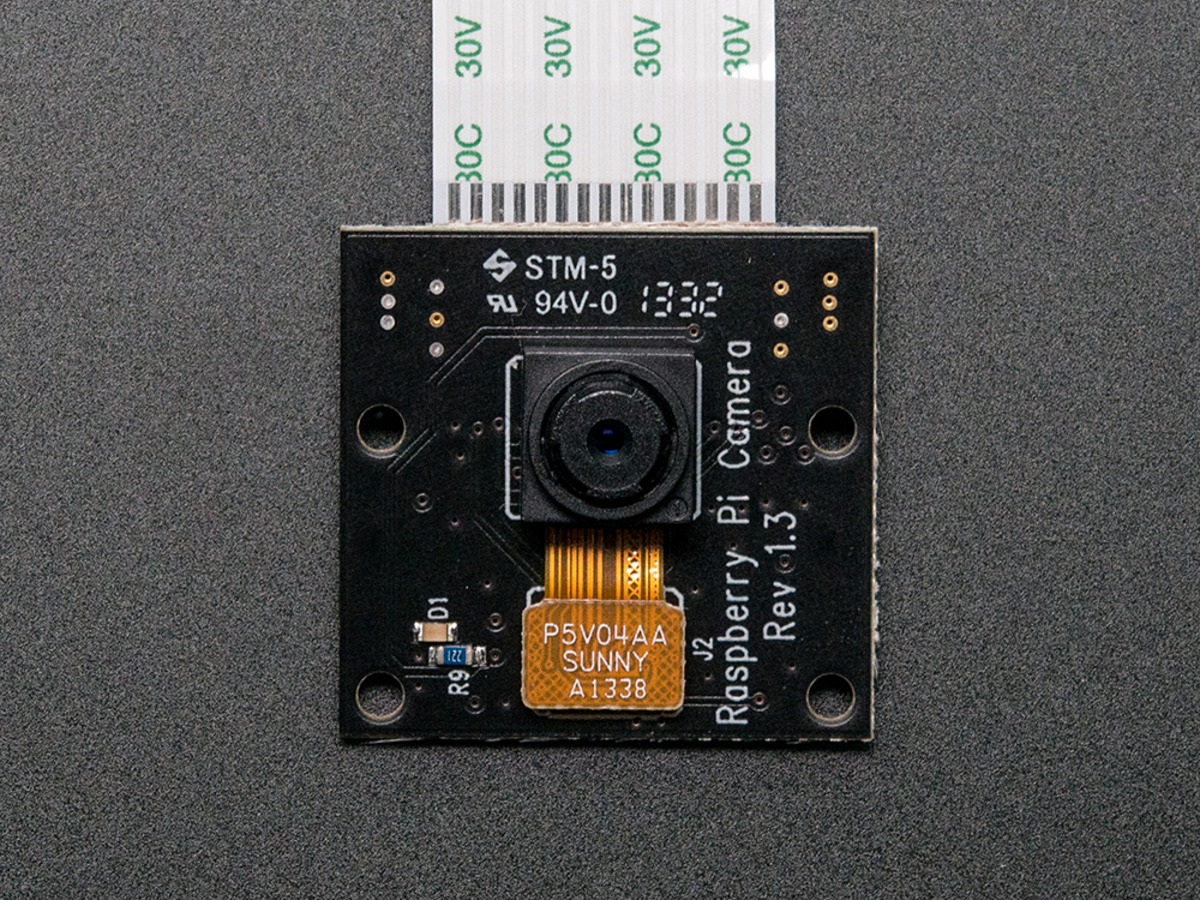
\includegraphics[width=0.5\textwidth]{fig/raspberry-pi-camera-noir.jpg}
\caption{Pi Cam Noir (Quelle: https://www.adafruit.com)}
\label{fig:PiCamNoir}
\end{figure}

\begin{table}[h]
\begin{tabular}{p{0.5\textwidth} | p{0.5\textwidth}}


 \textbf{Vorteile} & \textbf{Nachteile} \\ \hline
	 
\begin{itemize}
\item Relativ tiefe Anschaffungskosten
\item Analog Raspberry Pi Cam
\item Infrarot bei Tageslicht verwendbar, weniger empfindlich auf ändernde Lichtverhältnisse
\end{itemize}

 
 &
 
\begin{itemize}
\item Fester Fokus auf 1m
\item Relativ geringer Winkel mit 53.5°
\item Halterung muss erstellt werden
\item MIPI Schnittstelle erforderlich
\item Keine echten Farben, Erkennung derer unsicher
\end{itemize}

\end{tabular}
\end{table}

\begin{table}[h]
\begin{tabular}{p{0.5\textwidth}p{0.5\textwidth}}


 \textbf{Risiken} & \\ \hline
	 
\begin{itemize}
\item Fahrbahn kann in der Kurve nicht vollständig erfasst werden
\item Objekte können nicht vollständig erfasst werden
\item Kompatibilität zu Minicomputer eingeschränkt (Nur Rasp Pi und Banana Pi)
\end{itemize}
&
\begin{itemize}
\item Kein Autofokus: Scharfstellung nicht sichergestellt
\item Farben könnten nicht richtig erkannt werden
\item Höhere Anschaffungskosten ohne Garantie auf Erfolgsverbesserung
\end{itemize}

 
\end{tabular}
\end{table}

\pagebreak

%##############
\subsection{Webcam}

\begin{figure}[h!]%Position festigen
\centering
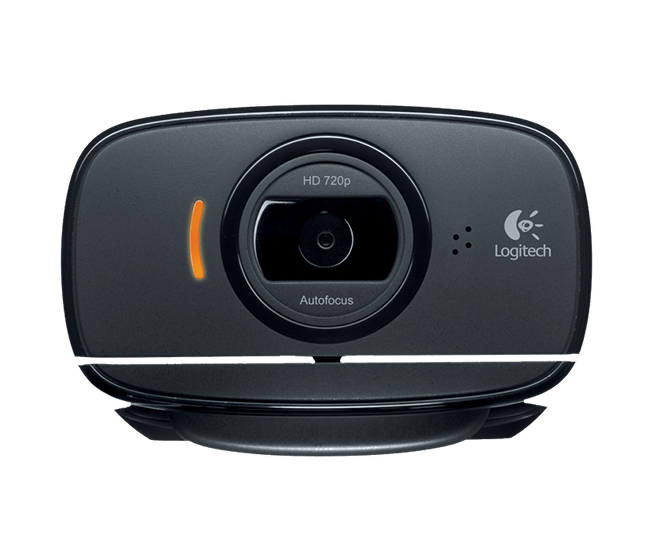
\includegraphics[width=0.5\textwidth]{fig/hd-webcam-c525-gallery.png}
\caption{Webcam (Quelle: http://www.logitech.com)}
\label{fig:Webcam}
\end{figure}

\begin{table}[h]
\begin{tabular}{p{0.5\textwidth} | p{0.5\textwidth}}


 \textbf{Vorteile} & \textbf{Nachteile} \\ \hline
	 
\begin{itemize}
\item Grosse Modellvielfalt
\item Autofokus
\item Grosser Blickwinkel mit ca 80° horizontal
\item USB-Universalschnittstelle
\item Halterung oftmals integriert
\end{itemize}

 
 &
 
\begin{itemize}
\item Höhere Anschaffungskosten
\item Kamerafunktionalitäten nur mit Herstellertreiber (proprietär)
\item Treiber meist nur für Windows erhältlich
\item Grössere Abmasse
\end{itemize}

\end{tabular}
\end{table}

\begin{table}[h]
\begin{tabular}{p{0.5\textwidth}p{0.5\textwidth}}


 \textbf{Risiken} & \\ \hline
	 
\begin{itemize}
\item Vorteile der Kamera können nicht genutzt werden
\item Kamerasystem zu gross, müsste zerlegt werden
\end{itemize}
&
\begin{itemize}
\item Hohe Kosten belasten Budget zu stark
\end{itemize}

 
\end{tabular}
\end{table}

\pagebreak